\documentclass[conference]{IEEEtran}
\IEEEoverridecommandlockouts
\usepackage{cite}
\usepackage{amsmath}
\usepackage{amssymb}
\usepackage{amsfonts}
\usepackage{algorithmic}
\usepackage{textcomp}
\usepackage{xcolor}
\usepackage{fancyhdr}
\usepackage{array}
\usepackage{caption}
\usepackage[shortcuts,acronym]{glossaries}
\usepackage{graphicx}
\usepackage[hidelinks]{hyperref}
\usepackage{multicol}
\usepackage{multirow}
\usepackage{subfigure}
\usepackage{listings}
\usepackage{color}
\usepackage{dirtree}

\definecolor{mygreen}{rgb}{0,0.6,0}
\definecolor{mygray}{rgb}{0.5,0.5,0.5}
\definecolor{mymauve}{rgb}{0.58,0,0.82}

\lstset{ 
backgroundcolor=\color{white},				% choose the background color; you must add \usepackage{color} or \usepackage{xcolor}; should come as last argument
basicstyle=\tiny\ttfamily,			        % the size of the fonts that are used for the code
breakatwhitespace=false,					% sets if automatic breaks should only happen at whitespace
breaklines=true,							% sets automatic line breaking
captionpos=b,								% sets the caption-position to bottom
commentstyle=\itshape\color{mygreen},		% comment style
deletekeywords={...},						% if you want to delete keywords from the given language
escapeinside={\%*}{*)},						% if you want to add LaTeX within your code
extendedchars=true,							% lets you use non-ASCII characters; for 8-bits encodings only, does not work with UTF-8
frame=single,								% adds a frame around the code
keepspaces=true,							% keeps spaces in text, useful for keeping indentation of code (possibly needs columns=flexible)
keywordstyle=\bfseries\color{blue},			% keyword style
morekeywords={*,...},						% if you want to add more keywords to the set
numbers=left,								% where to put the line-numbers; possible values are (none, left, right)
numbersep=4pt,								% how far the line-numbers are from the code
numberstyle=\color{mygray},					% the style that is used for the line-numbers
showspaces=false,							% show spaces everywhere adding particular underscores; it overrides 'showstringspaces'
showstringspaces=false,						% underline spaces within strings only
showtabs=false,								% show tabs within strings adding particular underscores
stepnumber=1,								% the step between two line-numbers. If it's 1, each line will be numbered
stringstyle=\color{mymauve},				% string literal style
tabsize=2,									% sets default tabsize to 2 spaces
}

\hypersetup{ colorlinks=true, citecolor=black, linkcolor=black, urlcolor=blue, }

\begin{document}

\title{Memory Centric Systems for AI Final Project Report: Play with DRAMsim3}
\author{\IEEEauthorblockN{2020314087 Sungmin Ryu}
        \IEEEauthorblockA{\textit{School of Electrical and Electronic Engineering}\\
                          \textit{Yonsei University}, Seoul, Korea}
}

\maketitle

\begin{abstract}
\emph{DRAMsim3}\cite{li2020dramsim3} is a cycle-accurate DRAM simulator, which faithfully models almost all aspects of modern DRAM, including the timings that we have covered, power consumption, etc.
In order to understand how \emph{DRAMsim3} works, I first made a trace-based memory controller.
With the memory controller, I tested the ResNet-18 traces changing scheduling methods of the simulator. 
Next, I built a timing memory controller to simulate simple memory timing test. 
Finally, I connected \emph{DRAMsim2} and \emph{gem5}\cite{binkert2011gem5} and then simulated AlexNet first convolutional layer.
With the simulation, I tested \emph{loop-unrolling} method which can reduce loop overhead. 
This report describes how to use the trace-based and timing memory controller, difference between FCFS and FR-FCFS scheduling, and some results of simulation.
\end{abstract}

\section{Introduction} \label{sec:introduction}
This report consists of three parts.
First, I explain how to use DRAMsim3 as a trace-based simulator and timing-based simulator respectively and show the results of the ResNet-18 trace simulation, in \emph{Section II}.
Second, I compare FCFS and FR-FCFS with the trace-based memory controller, in \emph{Section III}. 
In the last section, I describe the \emph{loop-unrolling} method and test the method with gem5-DRAMsim2.

\subsection{Overview of Project Sources}
\lstinputlisting[language=C++, title=- Source Tree -]{src/tree.txt}

Before we start, check the source tree above which contains main files and directories of this project.
\emph{DRAMsim3} is located in \emph{'ext'} and there are three main source files in \emph{'src'} directory: mem\_ctrler.h, mem\_ctrler.cc, and main.cc. 
The mem\_ctrler.h and mem\_ctrler.cc have some memory controller classes and functions respectively. 
In the main.cc, I can call the memory controllers and simulate trace-based simulation.  
All sources are available on my github(\url{https://github.com/WheatBeer/play_with_dramsim3}).

\subsection{DRAMsim3 Build Process}
During trace and timing simulation, I use DRAMsim3 as shared library(\emph{libdramsim3.so}) which is in ext/DRAMsim3(after library building).
One good thing about using the shared library is that we do not need to build every time the sources are changed. 
 I cloned \emph{DRAMsim3} in the \emph{'ext'} directory and changed DRAMsim3/src/configuration.cc to ext/configuration.cc, for my convenience(to save simulation outputs with output prefix).
After the change, I built \emph{DRAMsim3} and then \emph{libdramsim3.so} came out.

\lstinputlisting[language=C++, linerange={10-12}, firstnumber=10, title=- DRAMsim3 Headers -]{src/mem_ctrler.h}

Now, we are able to use memory systems in \emph{DRAMsim3} by adding some headers as above.
The 'common.h' includes \emph{Transaction} class which can take trace files, so the header is needed to make a trace-based memory controller. 
In addition, the 'dramsim3.h' is a required header to create \emph{DRAMsim3}'s \emph{MemorySystem}. 

\section{Memory Controller} \label{sec:mem_ctrler}
\subsection{Memory Controller Base Class}
\lstinputlisting[language=C++, linerange={22-43}, firstnumber=22, title=- Memory Controller Base Class -]{src/mem_ctrler.h}

The \emph{mem\_ctrler\_base\_t} class is the same as \emph{CPU} class in DRAMsim3/src/cpu.h(only the class's function and valable names are changed). 
The class has \emph{MemorySystem} pointer, \emph{'mem'}, which can use DRAMsim3 memory APIs in DRAMsim3/src/dramsim3.h. 
In src/main.cc, I can initiate the class's child classes(trace-based and timing memory controller) and get some outputs.

\subsection{Trace-based Memory Controller}
\lstinputlisting[language=C++, linerange={45-71}, firstnumber=45, title=- Trace-based Memory Controller Class -]{src/mem_ctrler.h}

In order to simulate trace memory requests, a trace-based memory controller is needed.  
The controller is already in DRAMsim3/src/cpu.h as \emph{TraceBaseCPU} class which is inherited from \emph{CPU} class, so users can use this by executing 'dramsim3main(executable file)' with a flag(e.g. -t trace.txt). 
However, to run this way, users have to put cycles(e.g. -c 100000) and the cycles do not guarantee the end of trace. 
For instance, the simulation is finished in the cycles, but traces may still remain.  
So, to track the last cycle, I made a new trace-based memory controller, \emph{trace\_mem\_ctrler\_t}, which is inherited from \emph{mem\_ctrler\_base\_t} class. 
The difference between \emph{trace\_mem\_ctrler\_t} class(new) and  \emph{TraceBaseCPU} class(original) is whether the last cycle can be tracked automatically. 
The new trace-based memory controller has some more functions and variables, such as \emph{is\_end()}, \emph{trace\_cnt}, and \emph{callback\_cnt}.

The way to track the last cycle is to count sending and receiving both and compare them. 
When sending transactions, \emph{trace\_cnt} is counted and when receiving callback(read and write), \emph{callback\_cnt} is counted.
The \emph{callback\_cnt} is incremented in the callback functions inside the controller and the increase of \emph{trace\_cnt} occurs at the \emph{tick()}, as you can see in the code below.

\lstinputlisting[language=C++, linerange={3-21}, firstnumber=3, title=- Trace-based Memory Controller's tick() -]{src/mem_ctrler.cc}

After all trace transactions are sent and \emph{DRAMsim3}'s \emph{MemorySystem} process the last transaction, \emph{callback\_cnt} becomes equal to \emph{trace\_cnt}. 
The \emph{is\_end()} function checks the end of the trace file and if \emph{trace\_cnt} and \emph{callback\_cnt} are the same. 

\lstinputlisting[language=C++, linerange={35-41}, firstnumber=35, title=- main.cc -]{src/main.cc}

In the main.cc, we can send all transactions in the trace file to the simulator and check whether the transaction processing is finished, using the \emph{is\_end()}.   

\lstinputlisting[linerange={1-15}, firstnumber=1, title=- The number of trace transations -]{src/trace_line.txt}

There are 8 ResNet-18 traces in the \emph{traces} directory.
The \emph{trace1} has 110272 transactions, of which READ transactions are 9920 and WRITE transactions are 100352.
In the output of \emph{trace1} simulation below, \emph{num\_reads\_done} and \emph{num\_write\_done} are the number of READ and WRITE transactions respectively. 
(There is 1 count difference at \emph{num\_reads\_done}, but I don't have enough time to debug.)
With the output, we can see that the number of cycles required to process all transactions is 559529(\emph{num\_cycles}).  

\lstinputlisting[linerange={1-9}, firstnumber=1, title=- Simulation Output(trace1) -]{src/fr_fcfs_trace1.txt}

To validate my trace-based memory controller, I use the original memory controller which name is \emph{TraceBaseCPU} in DRAMsim3/src/cpu.h. 
I put 559529 in cycle(-c 559529) and simulate \emph{trace1}, you can test as command below. 
After simulation, dramsim3.txt which is simulation output come out and the results are perfectly consistent with my results (even the \emph{1 count difference} is the same).   

\lstinputlisting[linerange={17}]{src/trace_line.txt}

\subsection{Timing Memory Controller}
A downside of trace-based simulation is it cannot simulate the real slowdown of an application, since the requests will arrive at the designated cycle no matter what. 
We can create a timing memory controller which has a fixed number of load buffer.
In this report, I only describe how to make the timing memory controller and how the controller works with infinite buffer. 

\lstinputlisting[language=C++, linerange={73-92}, firstnumber=73, title=- Timing Memory Controller Class -]{src/mem_ctrler.h}
\lstinputlisting[language=C++, linerange={23-55}, firstnumber=23, title=- Timing Memory Controller's Functions -]{src/mem_ctrler.cc}

The above memory controller, \emph{timing\_mem\_ctrler\_t}, has wrapper functions which include memory system functions in ext/DRAMsim3/src/dramsim3.h.
In the trace-based memory controller, \emph{WillAcceptTransaction()} and \emph{AddTransaction()}, which are memory system functions, are used inside the \emph{tick()}.
You can take this method in timing simulation.
Another way is to wrap these functions with \emph{will\_accept\_transaction} and \emph{add\_transaction} respectively and use them outside the controller.
For example, in your timing simulator, \emph{will\_accept\_transaction} should be called first to check whether DRAMsim3 can receive transactions.
If DRAMsim3 can accept the transactions, you can send memory requests through \emph{add\_transaction}.   
Next, you have to run \emph{tick()} for processing the transactions in \emph{DRAMsim3}.
The difference between these two methods is to schedule memory requests inside or outside the controller(I am currently looking for a suitable method in my research).

\lstinputlisting[language=C++, linerange={14-20}, firstnumber=14, title=- Memory Request Structure -]{src/mem_ctrler.h}

\begin{figure}
    \centering
    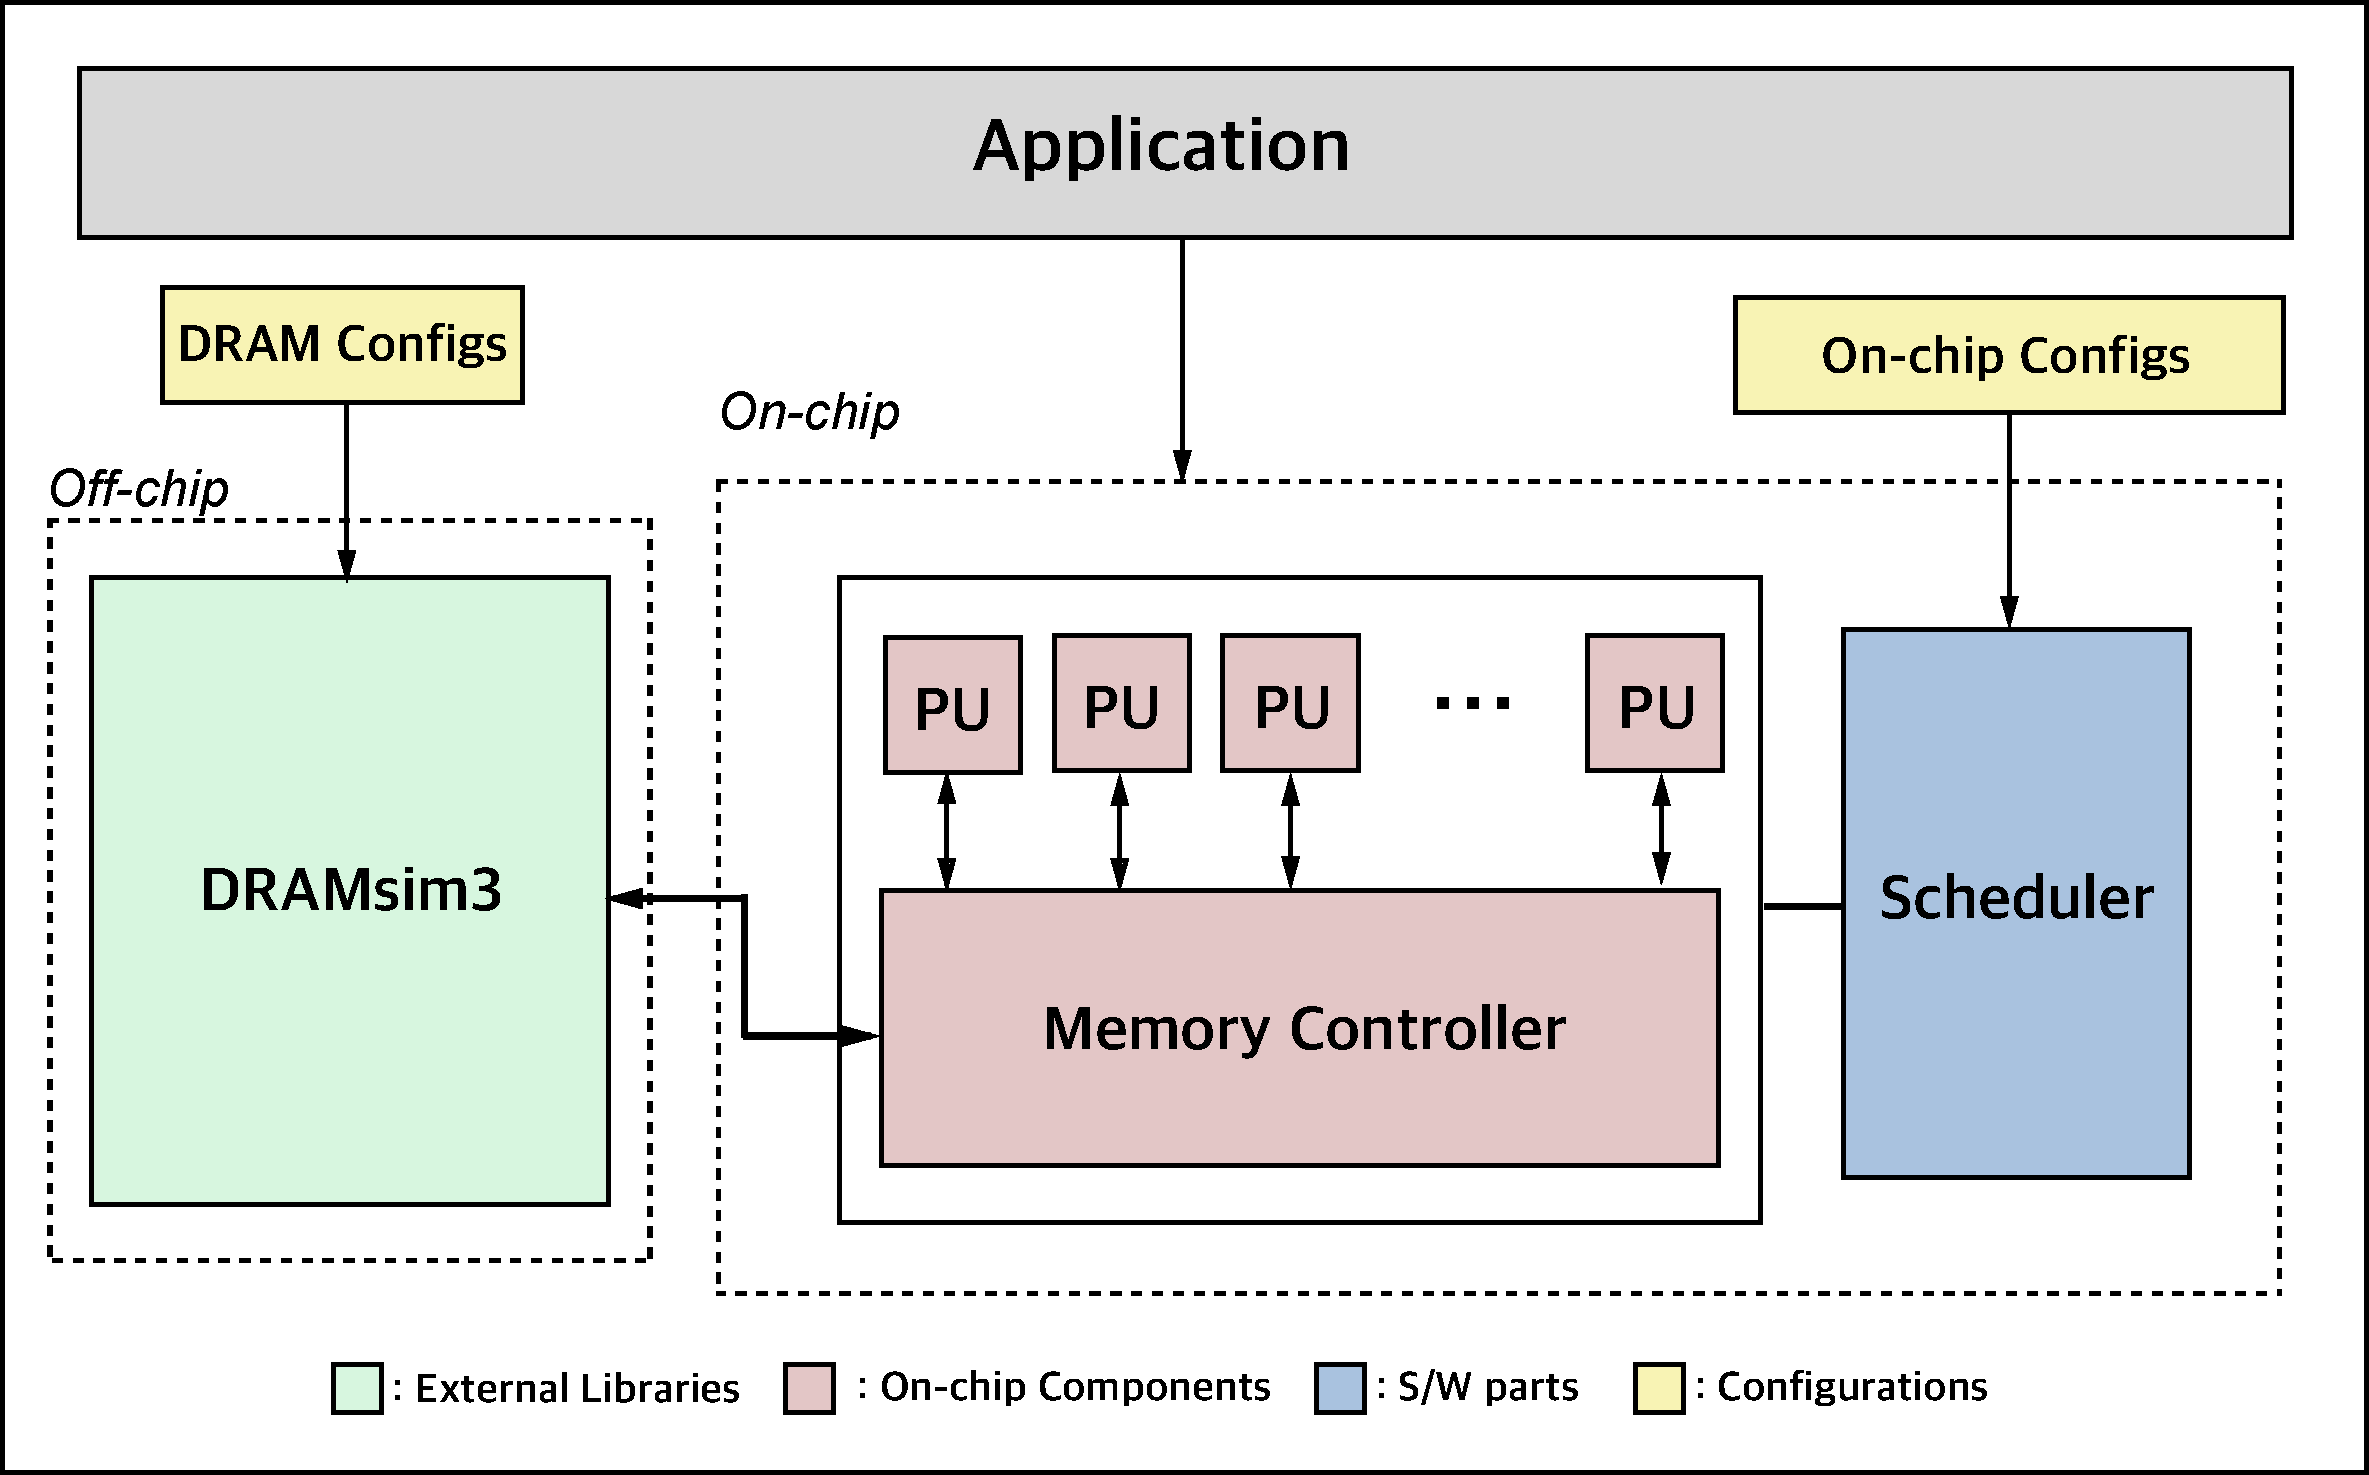
\includegraphics[width=1.00\linewidth]{image/example.pdf}
    \caption{Timing Simulation Example}
    \label{fig:tse}
\end{figure}

The \emph{timing\_mem\_ctrler\_t} has a queue which can contain memory requests(\emph{mem\_request\_t}).
The queue size can be fixed as needed.

To reduce description in the last section(\emph{gem5 with DRAMsim3}) and explain how the \emph{timing\_mem\_ctrler\_t} works, I use Fig.\ref{fig:tse} as an example.
When application is launched, PUs(Processing Units) send memory requests to the memory controller. 
If the memory controller queue has enough space, the memory requests are accepted and send to DRAMsim3. 
If not, the PU is stalled until queue can take the requests.
After DRAMsim3 processing, the memory controller receive processed address through callback functions.     
With the callback functions, memory controller should send data or message to PUs.
In \emph{gem5}, there can be various combinations of CPU and caches by configuration scripts. 

\section{DRAM Scheduler} \label{sec:dram_scheduler}
\subsection{FCFS vs FR-FCFS}
DRAMsim3 follows FR-FCFS(first-ready-first-come-first-serve) policy according to its github(\url{https://github.com/umd-memsys/DRAMsim3}). 
I change the policy to FCFS as follows.

\lstinputlisting[language=C++, linerange={178-196}, firstnumber=178, title=- FR-FCFS to FCFS -]{src/command_queue.cc}

DRAMsim3 memory system has two types of queue: transaction queue and bank command queue. 
The default value of transaction queue size is 32 and each bank has 8 command queue size.
From transaction queue to bank command queue, FCFS policy is applied. 
After commands sent to command queue, row-hit commands are served first following FR-FCFS.   

\subsection{Simulation Results and Analysis}

\begin{figure}
    \centering
    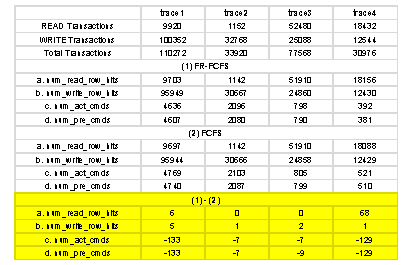
\includegraphics[width=1.00\linewidth]{image/dramsim3_1.pdf}
	\caption{Simulation Results(FR-FCFS vs FCFS)}
    \label{fig:simulation_result}
\end{figure}

I simulate ResNet-18 trace1-4 changing scheduling policy.
Fig. \ref{fig:simulation_result} is results of the simulation. 
The yellow box shows the subtracted values from FR-FCFS to FCFS.  
In most cases, row-hit ratio is higher when FR-FCFS scheduler is used than FCFS.
Since the traces have their own charateristics, the outputs are different for each trace.  

\section{Gem5 with DRAMsim2} \label{sec:gem5}
\subsection{Application Description}
\lstinputlisting[language=C++, linerange={7-31}, firstnumber=7, title=- AlexNet Conv1 Layer(Original) -]{src/origin.cc}
\lstinputlisting[language=C++, linerange={15-33}, firstnumber=15, title=- AlexNet Conv1 Layer(Unrolled) -]{src/unroll.cc}

I use the first convolutional layer in AlexNet and compare this with an unrolled version.
The original has 6 for-loop and each loop is increased by 1.
On the other hand, the unrolled version's inner most loop is counted by 4(S: filters' width).
Because of this, the unrolled version have 4 multiplication operations.
The applications run on gem5 8 TimingSimpleCPU(X86) cores with command below.

\lstinputlisting[linerange={3-8}, firstnumber=1, title=- gem5 Command Line -]{src/dramsim2.sh}
\subsection{Simulation Results and Analysis}

\begin{figure}
    \centering
    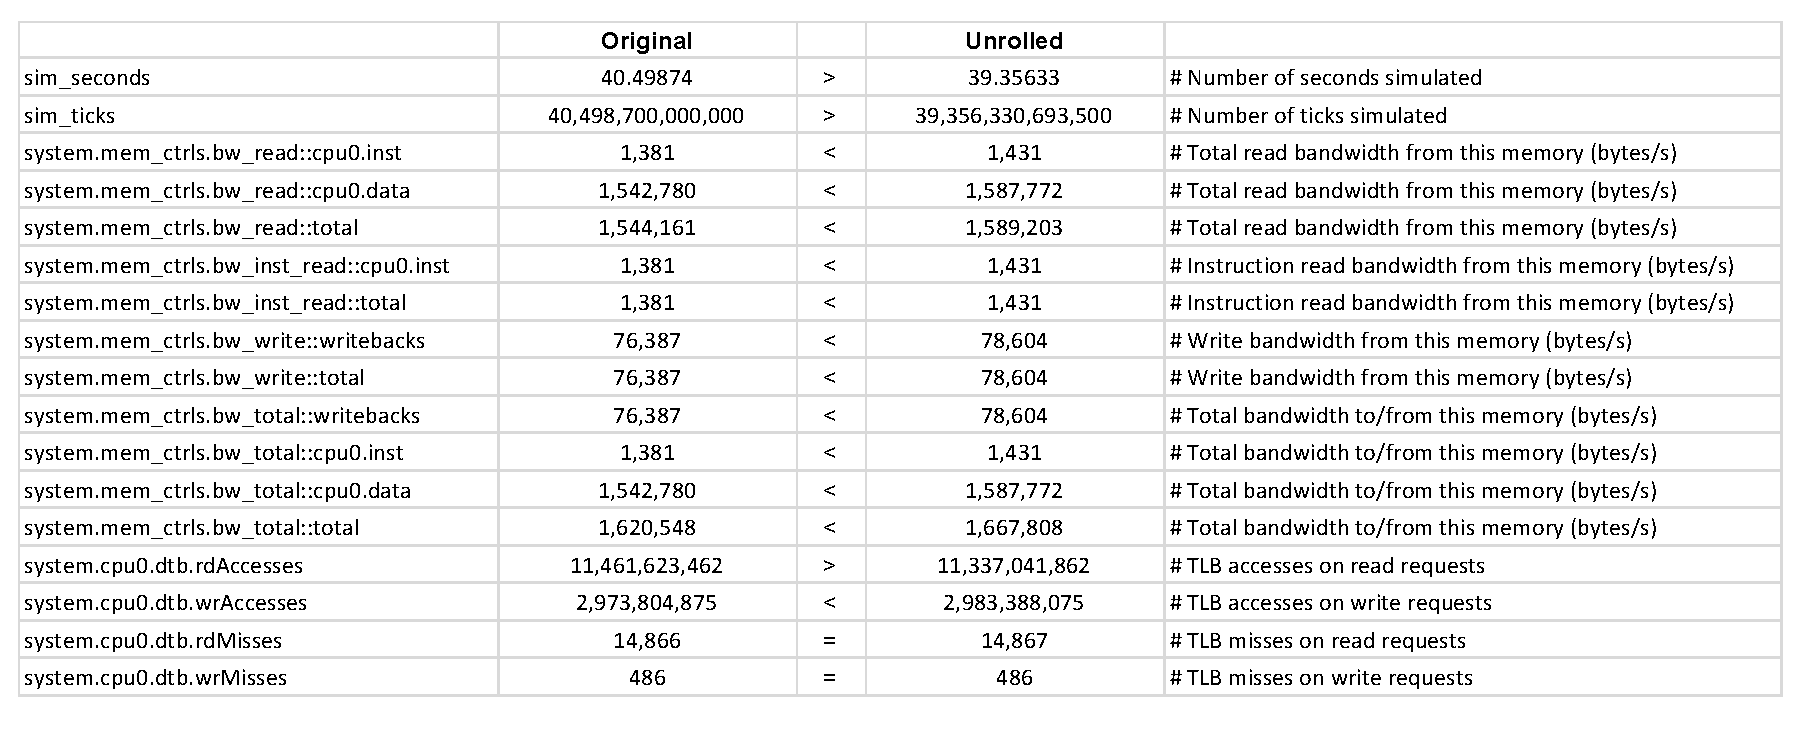
\includegraphics[width=1.00\linewidth]{image/m5out.pdf}
	\caption{Simulation Results(Original vs Unrolled)}
    \label{fig:m5out}
\end{figure}

Fig. \ref{fig:m5out} is results of the simulation. 
As expected, the unrolled test is finished faster than the original.
The reason of the difference of cycles is that the unrolled loop encounters branch instructions less than original.
At the \emph{system.mem\_ctrls.bw} parts in the results, all the unrolled outputs are larger than the original's.
Since the requests are almost same for both and the the unrolled test's taken time is shorter than original's, the unrolled version memory bandwidth numbers are larger than original's. 

\section{Conclusion} \label{sec:conclusion}
I tried to attach \emph{DRAMsim3} to \emph{gem5}, however, some problems came out.
At \emph{dramsim3::BaseDRAMSystem::ResetStats()}, which resets output stats, segmentation fault signal is detected.  
After fixing this, \emph{dramsim3::MemorySystem::ClockTick()} problem occured. 
Since I don't have enough time to debug this, I decided to use \emph{DRAMsim2} which is more stable than \emph{DRAMsim3}.
While working on this project, I was able to learn how DRAM works and how hardware simulators work.
In my future work, what I have learned from this project will be helpful a lot. 

% References
\bibliographystyle{references}
\bibliography{references}

\end{document}

